%% LyX 2.3.5.2 created this file.  For more info, see http://www.lyx.org/.
%% Do not edit unless you really know what you are doing.
\documentclass[12pt,english]{article}
\usepackage[T1]{fontenc}
\usepackage[utf8]{inputenc}
\usepackage{geometry}
\geometry{verbose,tmargin=2cm,bmargin=2cm,lmargin=2cm,rmargin=2cm}
\usepackage{fancyhdr}
\pagestyle{fancy}
\setlength{\parskip}{\smallskipamount}
\setlength{\parindent}{0pt}
\usepackage{babel}
\usepackage{refstyle}
\usepackage{float}
\usepackage{amsmath}
\usepackage{amssymb}
\usepackage{graphicx}
\usepackage{setspace}
\PassOptionsToPackage{normalem}{ulem}
\usepackage{ulem}
\setstretch{1.5}
\usepackage[unicode=true,pdfusetitle,
 bookmarks=true,bookmarksnumbered=false,bookmarksopen=false,
 breaklinks=false,pdfborder={0 0 1},backref=false,colorlinks=false]
 {hyperref}

\makeatletter

%%%%%%%%%%%%%%%%%%%%%%%%%%%%%% LyX specific LaTeX commands.

\AtBeginDocument{\providecommand\figref[1]{\ref{fig:#1}}}
\AtBeginDocument{\providecommand\eqref[1]{\ref{eq:#1}}}
\AtBeginDocument{\providecommand\subsecref[1]{\ref{subsec:#1}}}
\AtBeginDocument{\providecommand\algref[1]{\ref{alg:#1}}}
\floatstyle{ruled}
\newfloat{algorithm}{tbp}{loa}
\providecommand{\algorithmname}{Algorithm}
\floatname{algorithm}{\protect\algorithmname}
\RS@ifundefined{subsecref}
  {\newref{subsec}{name = \RSsectxt}}
  {}
\RS@ifundefined{thmref}
  {\def\RSthmtxt{theorem~}\newref{thm}{name = \RSthmtxt}}
  {}
\RS@ifundefined{lemref}
  {\def\RSlemtxt{lemma~}\newref{lem}{name = \RSlemtxt}}
  {}


%%%%%%%%%%%%%%%%%%%%%%%%%%%%%% Textclass specific LaTeX commands.
\newenvironment{lyxcode}
	{\par\begin{list}{}{
		\setlength{\rightmargin}{\leftmargin}
		\setlength{\listparindent}{0pt}% needed for AMS classes
		\raggedright
		\setlength{\itemsep}{0pt}
		\setlength{\parsep}{0pt}
		\normalfont\ttfamily}%
	 \item[]}
	{\end{list}}

%%%%%%%%%%%%%%%%%%%%%%%%%%%%%% User specified LaTeX commands.
% Hebrew does not work unless I use this. 
\usepackage{culmus}

\usepackage{fancyhdr}
\fancyhf{}               % Clear fancy header/footer
\fancyhead[C]{
\begin{otherlanguage}{English}
Technion, Faculty of Industrial Engineering and Management
\end{otherlanguage}
}   
\fancyfoot[C]{\thepage}  % Page number in Right footer
\makeatletter
\let\ps@plain\ps@fancy   % Plain page style = fancy page style
\makeatother
\newref{fig}{refcmd={\hyperref[#1]{Figure \ref{#1}}}}
\newref{tab}{refcmd={\hyperref[#1]{Table \ref{#1}}}}
\newref{eq}{refcmd={\hyperref[#1]{Eq. (\ref{#1})}}}
\newref{alg}{refcmd={\hyperref[#1]{Algorithem (\ref{#1})}}}

\makeatother

\begin{document}
\title{Introduction to Casual Inference - 097400\\
Winter 2021 - Project Report}
\author{Asaf Gendler 301727715 Shalev Shaer 305252520}

\maketitle
\newpage{}

\section{\uline{Introduction:}}

Over the last 20 years, genome-wide association studies (GWAS) have
established the association of thousands of genetic markers with phenotypes
of interest, and these studies have the potential to shed light on
essential scientific questions and to enable personalized medical
care. As new methods for analyzing GWAS emerge, the problem that arises
is that finding statistical association between genetic variants and
some outcome , could also identify some irrelevant associations due
to non genetic factors, and thus not necessarily indicate on a causal
relation. There are methods to remove those irrelevant associations,
however, they have no guarantee to ultimately remove them, thus the
main goal over the next years will be to move from statistical association
framework to causality framework, using the methods of this rising
field. While the best way to identify causality is to perform a randomized
controlled trail (RCT), this kind of trial is not possible when dealing
with genotypes of humans. Instead, we can identify causality throw
observational study of father-mother-offspring trios data-sets due
to the natural randomness of the recombination process of the offspring's
genes. The paper \cite{Bates_2020} that we are basing on suggests
a new analytic framework to identify causal effect of certain areas
in the genome over some outcome through hypothesis testing using Conditional
Randomized Tests(CRT). In this project we first review their methods
and their mathematical justifications and then suggest a new approach
to integrate randomness during training as well. We finish by showing
some initial results that suggest that such an approach can indeed
be useful.s

\section{\uline{Problem Formulation:}}

\subsection{Data-set Structure:}

To understand the problem, methods and the improvement we suggest,
we first have to formulate the problem mathematically. To do so, we
need to have a little bit of understanding of concepts in genetics,
that will help us better understand out data-sets. The human cells
have $36$ DNA strands organized into $23$ chromosomes pairs, In
each chromosome pair, one strand is inherited from the father and
one strand is inherited from the mother. Each one of this strands
is called a haplotype. The haplotype consists of a chain of links
called single-nucleotide polymorphisms or SNP. The reason their are
called so is that they can appear in the population in one of two
possible ways, therefore they can be encoded as binary variables which
can get the values of $0$ or $1$. See \figref{Hapoltypes_and_SNP}
for visualization of the described above.

\begin{figure}[H]
\begin{centering}
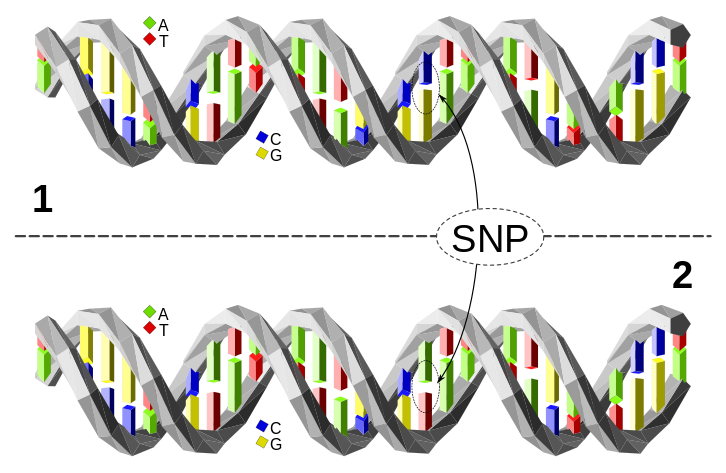
\includegraphics[width=0.5\textwidth]{figure1}
\par\end{centering}
\caption{\label{fig:Hapoltypes_and_SNP}An illustration of haplotypes and SNPs.
The chromosome pair consists of two DNA strands. Each strand is called
an haplotype. Each single link in the haplotype is called a SNP and
can take one of two forms in the population.}
\end{figure}

We consider a data-set of $n$ father-mother-offspring trios, where
for each one of them we have two haplotypes encodings of $p$ SNP's
values, all the haplotypes are of the same chromosome. The haplotypes
of the father will be denoted as $F^{a}$ and $F^{b}$, the mother's
as $M^{a}$ and $M^{b}$ , and the offspring, which is our test subject
as $X^{f}$ and $X^{m}$ as they are inherited from the father and
mother respectively. The data-set structure is thus as follows:
\[
\begin{array}{cc}
\begin{cases}
F^{a}=\left(\begin{array}{cccccc}
| & | &  &  &  & |\\
F_{1}^{a} & F_{2}^{a} & . & . & . & F_{p}^{a}\\
| & | &  &  &  & |
\end{array}\right)\in\left\{ 0,1\right\} ^{nxp}\\
 & \Longrightarrow\\
F^{b}=\left(\begin{array}{cccccc}
| & | &  &  &  & |\\
F_{1}^{b} & F_{2}^{b} & . & . & . & F_{p}^{b}\\
| & | &  &  &  & |
\end{array}\right)\in\left\{ 0,1\right\} ^{nxp}
\end{cases} & X^{f}=\left(\begin{array}{cccccc}
| & | &  &  &  & |\\
X_{1}^{f} & X_{2}^{f} & . & . & . & X_{p}^{f}\\
| & | &  &  &  & |
\end{array}\right)\in\left\{ 0,1\right\} ^{nxp}\\
\begin{cases}
M^{a}=\left(\begin{array}{cccccc}
| & | &  &  &  & |\\
M_{1}^{a} & M_{2}^{a} & . & . & . & M_{p}^{a}\\
| & | &  &  &  & |
\end{array}\right)\in\left\{ 0,1\right\} ^{nxp}\\
 & \Longrightarrow\\
M^{b}=\left(\begin{array}{cccccc}
| & | &  &  &  & |\\
M_{1}^{b} & F_{2}^{b} & . & . & . & F_{p}^{b}\\
| & | &  &  &  & |
\end{array}\right)\in\left\{ 0,1\right\} ^{nxp}
\end{cases} & X^{m}=\left(\begin{array}{cccccc}
| & | &  &  &  & |\\
X_{1}^{m} & X_{2}^{m} & . & . & . & X_{p}^{m}\\
| & | &  &  &  & |
\end{array}\right)\in\left\{ 0,1\right\} ^{nxp}
\end{array}
\]

For easier notation we will denote the offsprings' matrix as $X=X^{f}+X^{m}$.
The $i$-th row of this matrix $X^{\left(i\right)}$ corresponds to
the haplotypes of the $i$-th subject, and the $j$-th column $X_{j}$
corresponds to the $j$-th SNP of all the subjects. We also denote
$A=\left\{ F^{a},F^{b},M^{a},M^{b}\right\} $ as the set of all parents
haplotypes (A as a short for ancestors).

\subsection{The goal}

Our main goal is to establish causality in the Trio design, in a rigorous
statistical sense. more precisely, we want to examine a causal connection
between a SNP $X_{j}$ or a group of SNPs $X_{C}=\left\{ X_{j}:j\in C\right\} $
to some phenomena or outcome $Y$. Differently from the main casual
problems that we saw in the course, where the goal was to calculate
the ATE or the ATT, our problem is only a binary problem that tries
to answer the question whether or not there is a causal connection,
and doesn't try to estimate it's value. Mathematically we formulate
the problem as a hypothesis testing problem as follows: given the
examined SNP $X_{j}$ and some outcome $Y$ we want to test the null
hypothesis:
\begin{align}
H_{0}:X_{j} & \perp\!\!\!\perp Y\label{eq:1}
\end{align}

which means that this SNP and the outcome are statistically independent.
Rejecting the null hypothesis will deduce that there is a statistical
connection between the two, however, as we saw in the course statistical
dependency and high correlation does not necessarily indicate a causal
effect. For example, take $Z$ to be some unobserved external variable
that has a high casual effect on the outcome $Y$. Consider the case
where the data-set contains two groups of populations, one group which
tends to have the SNP $X_{j}$ with a value of $1$ and also tends
to practice $Z$, and the other group which tends to have the SNP
$X_{j}$ with a value of $0$ and also doesn't tend to practice $Z$.
As a result, when testing the null hypothesis we suggested, we will
probably reject it and find a statistical connection between $X_{j}$
and $Y$, however, this relation was caused due the the correlation
between $X_{j}$ and $Z$, and the effect of $Z$ on $Y$, and no
due to a causal effect of $X_{j}$ on $Y$. $Z$ is in fact a hidden
confounder as we saw in the course, and the causal graph will look
like in \figref{Hidden_Confounder}, which doesn't let us identify
a causal effect of $X_{j}$ on $Y$.

\begin{figure}[H]
\begin{centering}
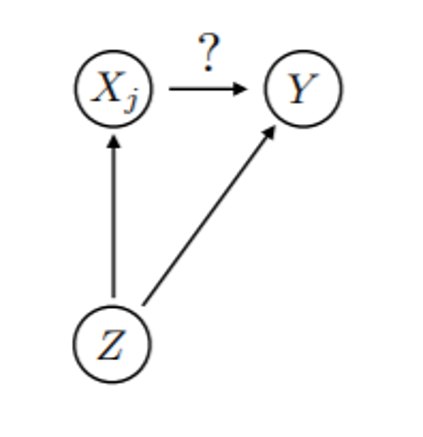
\includegraphics[width=0.25\textwidth]{figure2}
\par\end{centering}
\caption{\label{fig:Hidden_Confounder}A possible causal graph. In this scenario
we can't identify a causal connection between $X_{j}$ and $Y$ without
observing $Z$}
\end{figure}

As a result if we want to examine a causal effect, we need to do something
smarter, as suggested in the next topic.

\subsection{Identifying Causality\label{subsec:Identifying-Causality}}

To solve the problem of some external unobserved hidden confounders,
we need to address the recombination process of an offspring haplotypes
from his parents haplotypes. Remember that the offspring has two haplotypes,
one of them is a recombination of the two haplotypes of the father
and the other is a recombination of the two haplotypes of the mother,
an example for such a recombination can be seen in \figref{Recombination_Process}
.

\begin{figure}[H]
\begin{centering}
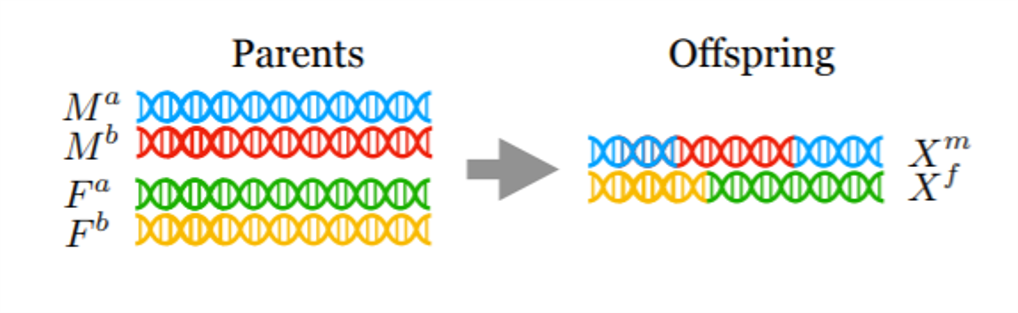
\includegraphics[width=0.5\textwidth]{figure4}
\par\end{centering}
\caption{\label{fig:Recombination_Process}One offspring's haplotype is a recombination
of the father's haplotypes and the other is a recombination of the
mother's haplotypes}
\end{figure}

The crucial point for understanding, is that this recombination is
a completely random process, with a known generation mechanism that
can be simulated. Basically it means that given the haplotypes of
the parents, we can stochastically model the generation process of
the offspring haplotypes, simulate it, sample from it, etc. Mathematically
it means that the distribution of $X_{j}$ and actually all the SNPs
is known given the parents haplotypes, which we denoted as the set
$A$. From considerations of space, we won't fully detail the mathematical
model of the recombination process, it is detailed in the paper and
was implemented by us in python.

The main advantage of the randomness of the offspring's haplotypes
recombination process is that if we go back to the scenario depicted
in \figref{Hidden_Confounder}, the causal graph should actually be
depicted as in \figref{Back_Door}.

\begin{figure}[H]
\begin{centering}
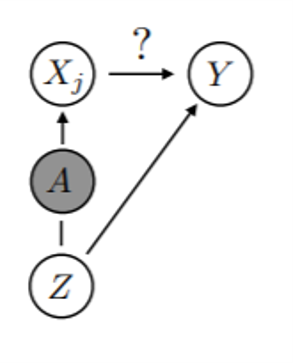
\includegraphics[width=0.25\textwidth]{figure3}
\par\end{centering}
\caption{\label{fig:Back_Door}The true casual graph, $X_{j}$ is effected
by $Z$ only through $A$ and thus $A$ satisfies the backdoor criterion}
\end{figure}

What we see is that the external hidden confounder $Z$ has a causal
effect on $X_{j}$ only through $A$, basically it means that any
external hidden confounder can effect the parents haplotypes, but
if we have observed them, then from there one the offspring haplotypes
can be effected only by them and not by any unobserved hidden confounder.
Understanding this, then instead of checking hypothesis \eqref{1},
we will instead check the following null hypothesis:
\begin{equation}
H_{0}:X_{j}\perp\!\!\!\perp Y|A\label{eq:2}
\end{equation}
The main theorem of the paper shows that checking \eqref{2} is equivalent
for checking the following:
\begin{equation}
H_{0}:X_{j}\perp\!\!\!\perp Y|A,Z\label{eq:3}
\end{equation}
where $Z$ is any external unobserved variable. What we see here is
basically the backdoor adjustment criterion which we saw in the course,
the set $A$ satisfies the backdoor criteria, corresponding to the
causal graph in \figref{Back_Door}, and thus conditioning on him
is enough to identify causality between $X_{j}$ and $Y$. 

\subsection{limitations}

From what we have showed in \subsecref{Identifying-Causality}, we
can deduce that if we have found a strong statistical connection between
$X_{j}$ and $Y$ conditioned on $A$, which basically means that
we will reject the null hypothesis \eqref{2}, is has to mean that
there is a causal effect between $X_{j}$ and $Y$. However, this
is not precisely the case. We have said that the recombination process
of the offspring's haplotypes is random conditioned on the parents,
which is true, but the SNPs themselves for example, $X_{j}$ and $X_{k}$
are not independent on each other given the parents haplotypes $A$.
This is due to the way the recombination occurs which we haven't discussed
in details here but in short, the recombination tends to keep large
chains of SNPs from the parents' haplotype, together in the offspring's
haplotype. These dependencies can make the causal graph look like
at \figref{SNP_dependencies} for example.

\begin{figure}[H]
\begin{centering}
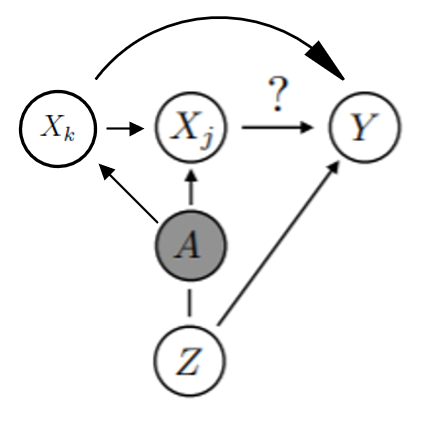
\includegraphics[width=0.25\textwidth]{figure5}
\par\end{centering}
\caption{\label{fig:SNP_dependencies}SNPs can be dependent on each other given
the parent haplotypes $A$, thus $A$ itself doesn't satisfy the backdoor
criterion anymore.}
\end{figure}

Analogously to our insight on the external counfounder $Z$, if we
reject hypothesis \eqref{2}, it could either mean that $X_{j}$ indeed
has an effect on $Y$ or that some other SNP actually caused the effect.
To deal with this issue, we will have to condition on all the other
SNPs there we are not checking, and define a new null hypothesis:
\begin{equation}
H_{0}:X_{j}\perp\!\!\!\perp Y|A,X_{-j}\label{eq:4}
\end{equation}
where $X_{-j}$ denotes all other SNPs besides $X_{j}$. Still, Hypothesis
\eqref{2} that from now on we will call the global casual null hypothesis,
has its benefits. This hypothesis testing still helps us find whether
or not there is some SNP on the pair of haplotypes that might effect
the outcome $Y$. If we reject the global null, it doesn't necessarily
means that $X_{j}$ has an effect on $Y$ but it does mean that some
SNP or a group of SNPs on the pair of haplotypes does have an effect.
On the other hand, accepting the global null means not only that $X_{j}$
doesn't have an effect but that actually all the SNPs on that haplotypes
pair doesn't have an effect. This is why we call this hypothesis the
global null, as it helps us to identify global causal effect between
a pair of haplotypes and an outcome $Y$. If we want to further localize
which SNP or group of SNPs actually caused the effect, we will need
to use \eqref{4} which is therefore called the local casual null
hypothesis. To check the local null we will have to know the distribution
of $X_{j}$ conditioned on his parents haplotypes, and all the other
SNPs. This is possible, and the paper details how to do so, however,
because this makes the generation procedure much more complicated,
and because our improvement can be cooperated with both the global
null and the local null, we will deal with only the global null from
now on.

We also remark that a few environmental factors of the parents can
affect the inheritance process, such as the exposure of a parent to
radiation, which changes the distribution of the offspring by increasing
the frequency of mutations. This factors will of course break the
backdoor criteria satisfied by $A$, however, those factors are very
rare and can be neglectable most of the times.

\section{\uline{Methods for solution:}}

Now that we have understood which null hypothesis we want to check,
let's discuss about the method to check it. We are going to check
the global null hypothesis in the most generalized way, that is, examine
the influence of a group of SNPs as follows:
\begin{align}
H_{0} & :X_{C}\perp\!\!\!\perp Y|A\nonumber \\
 & X_{C}=\left\{ X_{j}:j\in C\right\} \label{eq:5}
\end{align}

In order to do so, the paper suggests to use a version of the conditional
randomization test suggested in \cite{Cand_s_2018} and calls it the
Digital Twin Test (DTT). We will not proof the validity of the test
but only explain how in works. This test is useful when you want to
check a conditional hypothesis and you know how so sample from the
conditional probability, which is exactly our case. We will describe
the test in a more machine learning approach for better understanding
of our improvement. First we take the data and split in into training
and test sets. Then we fit some model between all the features, which
are the SNPs in our case, $X_{C}$ and $X_{-C}$ to the outcome $Y$.
We then calculate some error statistic $T$ of the model on the test
data, for example the MSE, and denote the value as $t^{*}$. Notice
that this statistic $T$ can in fact be any statistic we want (even
doesn't have to integrate machine learning methods) and the validity
of the test will still hold. Next, using our knowledge of the offspring's
haplotypes given the parents haplotypes, we generate for each pair
of parents in the test set $K$ digital offsprings (They are like
digital twins of the original offspring hence the name of the test),
effectively creating $K$ new test sets, and compute our statistic
$T$ on each one of them, each result denoted as $t_{j}$. The critical
point here is that when we create the digital offsprings, we only
take the part $\widetilde{X}_{C}$ that we want to examine from it,
and put in instead of the original $X_{C}$ while leaving the other
SNPs intact. At the end of the process we will have $K$ values $\left\{ t_{1},...,t_{k}\right\} $
and the original value $t^{*}$. All that is left to do is calculate
the relative position of $t^{*}$ among $\left\{ t_{1},...,t_{k}\right\} $
values (for example$\left(0.1\right)$), this will be our p-value
for the test (the test is rejected for any $\alpha$ that is higher
than the p-value). The reasoning behind this test, is that if the
group $X_{C}$ indeed has a statistical association with $Y$ (and
our model is well fitted), than by generating new digital offsprings
with different values of $X_{C}$, the outcome values predicted by
the model will change dramatically, hence the original error statistic
will be relative small compared to the others and we will get a small
p-value (which is s strong evidence for rejecting). On the contrary,
if the value of $X_{C}$ doesn't have any influence on the outcome,
we expect the model to predict more or less the same outcome values
just as before, hence $t^{*}$ shouldn't be small compared to $\left\{ t_{1},...,t_{k}\right\} $
and the p-value will be high, thus we will accept the null hypothesis.
a summary of the algorithm is presented in \algref{The-Digital-Twin}

\begin{algorithm}[H]
\begin{itemize}
\begin{singlespace}
\item Input: data $X$, outcome $Y$, parental data $A$, region $C$, number
of iterations $K$
\end{singlespace}
\end{itemize}
\begin{enumerate}
\begin{singlespace}
\item \textbf{Split} the data into train and test sets, and fit a model
$f\left(X_{C},X_{-C}\right)$ between the SNPs and the outcome on
the train data.
\item \textbf{Compute} the error test statistic on the test data:
\[
t^{*}=T\left(f\left(X_{C},X_{-C}\right),Y\right)
\]
\item \textbf{for} $k=1,...,K$ \textbf{Do}:
\end{singlespace}
\begin{enumerate}
\begin{singlespace}
\item \textbf{Sample} the digital twins $\widetilde{X}$ based on the parents
using the known $P\left(X|A\right)$ and put $\widetilde{X}_{C}$
instead of the original $X_{C}$.
\item \textbf{Compute} the error test statistic using the digital twins:
\[
t_{k}=T\left(f\left(\widetilde{X}_{C},X_{-C}\right),Y\right)
\]
\textbf{end}
\end{singlespace}
\end{enumerate}
\begin{singlespace}
\item \textbf{Compute} the quantile of the true statistic $t^{*}$ among
the digital twin statistics $\left\{ t_{1},...,t_{k}\right\} $
\end{singlespace}
\end{enumerate}
\begin{lyxcode}
\begin{singlespace}
\textrm{
\[
p_{val}=\frac{1+\sum_{i=1}^{K}\mathbb{I}\left\{ t_{i}\leq t^{*}\right\} }{K+1}
\]
}
\end{singlespace}
\end{lyxcode}
\caption{\label{alg:The-Digital-Twin}The Digital Twin Test}

\end{algorithm}


\section{\uline{Extension}}

\subsection{general}

Conditional Randomized Test (CRT) methods, such as the one we have
described in the Digital Twin Test are now common in order to test
hypothesis. CRT methods sample from a conditional distribution (in
our context it was $P\left(X_{C}|A\right)$ ) to create a \textquotedbl fake\textquotedbl{}
sample $\widetilde{X}_{C}$, and use the fake sample \textbf{only}
in the test (as a counter sample). We suggest to involve the fake
data $\widetilde{X}_{C}$ in the learning process as well (we can
get infinite samples of $\widetilde{X}_{C}$ as we sample from a known
distribution) in order to increase the power of the test or to decrease
the false detection rate. In this section we will combine $\widetilde{X}_{C}$
in a binary classifier, and examine whether the CRT give good results
or not.

\subsection{The proposed method}

Our proposed method is as follow: First, we create the fake data $\widetilde{X}$
by sampling the desired region $C$ from $P\left(X|A\right)$ and
substitute it with the desired region in $X$ . Then we concatenate
the outcome $Y$ once with $X$ and once with $\widetilde{X}$ , thus
creating real data and fake data. We add labels to each one of this
data sets, the real data gets the label $"1"$ and the fake data the
label $"0"$. We then train a binary classifier with the both the
real and fake data that tries to extinguish who is real and who is
not. The $T$ statistic in the CRT, which liked said before can be
any statistic, will now be the sum of the probabilities of getting
$"1"$ in the output of the classifier. The full algorithm is described
below.

\begin{algorithm}[H]
\begin{itemize}
\begin{singlespace}
\item Input: true data $X$, outcome $Y$, parental data $A$, binary classifier
, region $C$, number of iterations $K$
\end{singlespace}
\end{itemize}
\begin{enumerate}
\begin{singlespace}
\item \textbf{Create} $\widetilde{X}$ by sampling the digital twins like
in DTT $\widetilde{X}=\left(\widetilde{X}_{C},X_{-C}\right)$
\item \textbf{Create} the training data by concatenating $Y$ to $X$ and
to $\widetilde{X}$, and add the label $"1"$ to $X$ and $"0"$ to
$\widetilde{X}$
\item \textbf{Fit} the classifier with both $\left(X,Y,1\right)$ and $\left(\widetilde{X},Y,0\right)$
as one training set
\item \textbf{Compute} the test statistic on the test data: 
\[
t^{*}=-\sum_{i\in Test}P\left(classifier(x_{i},y_{i})=1\right)
\]
\item \textbf{for} $k=1,...,K$ \textbf{Do}:
\end{singlespace}
\begin{enumerate}
\begin{singlespace}
\item \textbf{Sample} the digital twins $\widetilde{X}$ based on the parents
using the known $P\left(X|A\right)$ and put $\widetilde{X}_{C}$
instead of the original $X_{C}$.
\item \textbf{Compute} the test statistic using the digital twins:
\[
t_{k}=-\sum_{i\in Test}P\left(classifier(\tilde{x}_{i},y_{i})=1\right)
\]
\end{singlespace}
\end{enumerate}
\begin{description}
\begin{singlespace}
\item [{end}]~
\end{singlespace}
\end{description}
\begin{singlespace}
\item \textbf{Compute} the quantile of the true statistic $t^{*}$ among
the digital twin statistics$\left\{ t_{1},...,t_{k}\right\} $
\end{singlespace}
\end{enumerate}
\begin{lyxcode}
\begin{singlespace}
\textrm{
\[
p_{val}=\frac{1+\sum_{i=1}^{K}\mathbb{I}\left\{ t_{i}\leq t^{*}\right\} }{K+1}
\]
}
\end{singlespace}
\end{lyxcode}
\caption{\label{alg:The-Digital-Twin-extended}The Digital Twin Test with binary
classifier}
\end{algorithm}

The reasoning behind our new proposal is as follows. If the set of
SNPs $X_{C}$ has a large influence on the outcome $Y$, the we expect
our classifier to train well, and be able to distinguish well between
real examples and the fake ones. In this case, when we will generate
the digital twins on the test set, the classifier will tend to give
higher probabilities to the original data over the generated one.
On the contrary, if the SNPs doesn't influence $Y$ at all, than our
trained classifier will act poorly, not able to distinguishing between
real and fake, hence the probabilities it will give to the digital
twins during test will be more or less the same to the probabilities
on the original set.

\section{\uline{Simulations and Results:}}

First, let us describe the settings. We create a synthetic population
of $n=250$ parent-child trios and generate an outcome coming from
a sparse regression model $Y^{\left(i\right)}=\beta^{T}X^{\left(i\right)}+v$
where $v\sim N(0,1)$. We use $p=100,150$ SNPs from a chromosome
with a width of $50$ Mb, and $\beta$ is sparse and has only $10$
non zeros entries of equal strength. We used four different signal
strength $c=1,2,3,4$, and for every value of $c$ we used the suggested
algorithm $20$ times. We choose Quadratic Discriminant Analysis (QDA)
as our classifier. These experiments demonstrate a situation of a
causal region, therefore we expect low p-values. We plot a plot-box
for the extracted p-values for every setting as can be seen in \figref{p100}
and \figref{p150}. As we can see, our method behave as expected -
the higher the signal strength the smaller the p-value and the narrower
the standard deviation of the p-values. Furthermore, the more SNPs
there are (the greater the $p$), the higher the p-values and wider
the standard deviation. The original DTT on this setting always results
in a minimal close to zero p-value so we didn't plot it as it does
not bring more information than this mention. For a final experiment
we produce the outcome $Y$ from a random distribution $N(0,1)$,
and ran the suggested algorithm with QDA classifier. The results are
in \figref{noisy_output}. We can see that for a noisy outcome, unrelated
to the SNPs, the p-values are high and with high standard deviation,
as expected.

\begin{figure}[H]
\begin{centering}
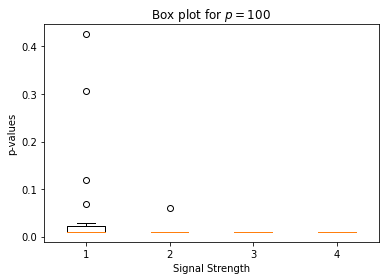
\includegraphics[width=0.5\textwidth]{p100}
\par\end{centering}
\caption{\label{fig:p100}A box plot for $p=100$ and $k=10$}
\end{figure}

\begin{figure}[H]
\begin{centering}
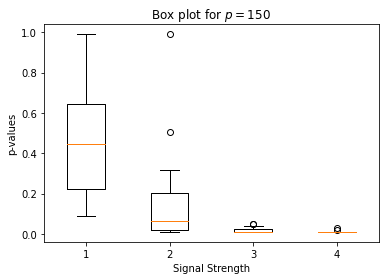
\includegraphics[width=0.5\textwidth]{p150}
\par\end{centering}
\caption{\label{fig:p150}A box plot for $p=150$ and $k=10$}
\end{figure}

\begin{figure}[H]
\begin{centering}
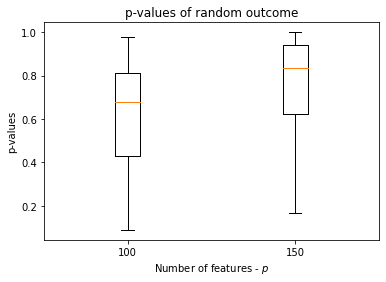
\includegraphics[width=0.5\textwidth]{noisy_outcome}
\par\end{centering}
\caption{\label{fig:noisy_output}A box plot for $p=100$ , $p=150$ and a
noisy output $Y$ unrelated to the SNPs}
\end{figure}


\section{\uline{Conclusion and Future Work:}}

Our method does not outperform the DTT as described above, but it
does work well and behave as expected. The main goal of this project
was to examine whether our idea to use $\widetilde{X}$ in the training
process make sense or not, and it seems that it does. For future work
one can consider involve $\widetilde{X}$ in more complex methods
(e.g Neural Networks) and check whether it increases the power and
\textbackslash{} or decrease the false detection rate. 

It is important to note that although we didn't test our method with
the local causal null hypothesis, we expect similar result as the
framework is the same and only the conditional sampling procedure
changes. Another aspect that both us and the paper didn't investigate
is the use of multiple hypothesis testing methods, such as FDR, to
unite examining of different SNPs regions into one more powerful test.
Of course that our method can be extended to this filed as well, as
it is generic.

\bibliographystyle{IEEEtran}
\bibliography{IEEEabrv,IEEEexample,IEEEfull,Candes,main_paper}

\end{document}
